\documentclass[11pt,a4paper]{jsarticle}
%
\usepackage[english]{babel}
\usepackage{amsmath,amssymb}
\usepackage{bm}
\usepackage{graphicx}
\usepackage{ascmac}
\usepackage{url}
%
\setlength{\textwidth}{\fullwidth}
\setlength{\textheight}{39\baselineskip}
\addtolength{\textheight}{\topskip}
\setlength{\voffset}{-0.5in}
\setlength{\headsep}{0.3in}
%
\newcommand{\divergence}{\mathrm{div}\,}
\newcommand{\grad}{\mathrm{grad}\,} 
\newcommand{\rot}{\mathrm{rot}\,} 
%
\pagestyle{myheadings}
\markright{\footnotesize Muography SiMulator (MSM)}

\title{Usage of Muography SiMulator (MSM)}
\author{Ryuichi Nishiyama}
\date{23 July 2015, revised on 30 March 2020}

\begin{document}

\maketitle

\section{Muography SiMulator (MSM)}
Muography SiMulator (MSM) is developed to perform a full 3D Monte Carlo simulation of 
particle transportation for the purpose of muography (muon radiography). One can realize 
any shape of mountain and detectors in the computational region and inject any type of particles
following energy spectrum model. This program is based on Geant4.10 The source code is 
extended from the novice program in Geant4.

This program was used in the calculation of the flux of background noise particles in muography experiments. The results is reported in Nishiyama et al (GJI, 2016 attached in the same directory). This work discuses the abudance of low-energy paritlces (protons, electrons and muons)  which mimic trajectories of muons passing through the target mountain. These low-energy particles could cause huge systematic uncertainty in muography experiments if appropreate measures are not taken.

\begin{figure*}
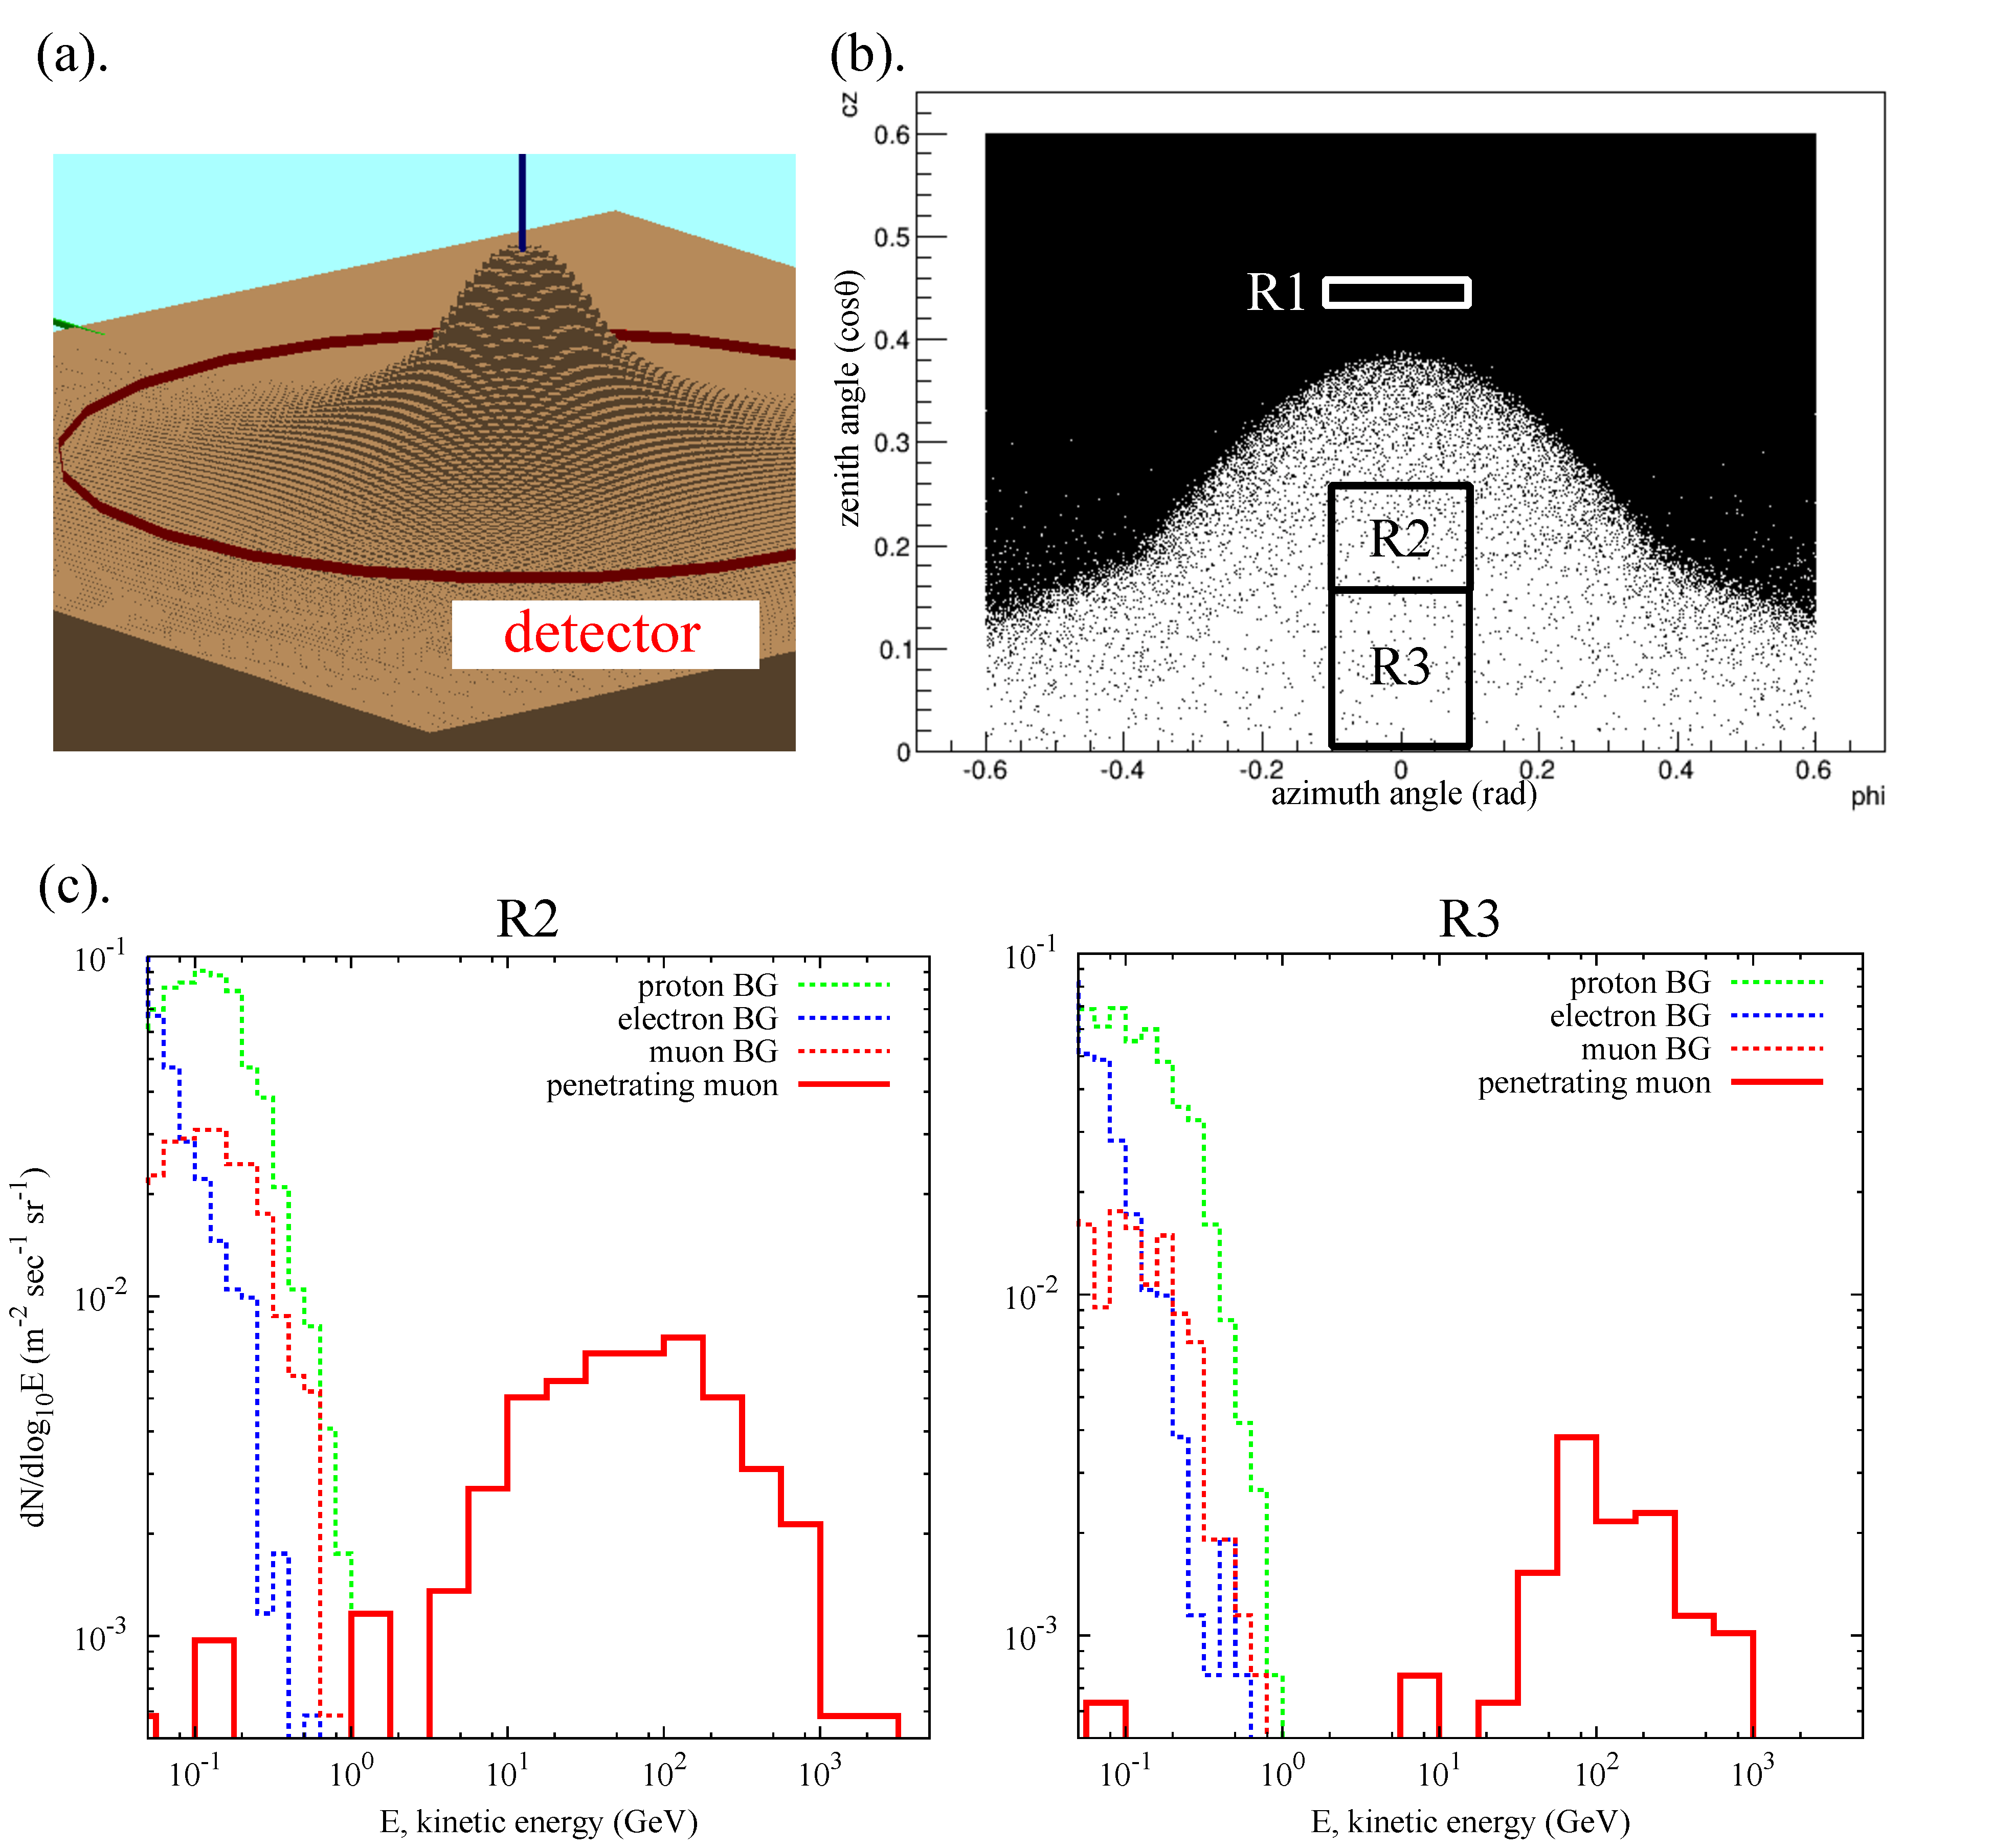
\includegraphics[width=120mm]{fig-geant4.eps}
\caption{(a) Virtual mountain and detector constructed in GEANT4 computational space. 
(b) Angular distribution of particles arriving at the virtual detector, showing three angular regions R1, R2 and R3 defined 
for quantitative analysis. (c) Number histogram of particles arriving at the virtual detector. The energy distributions of 
the penetrating muons and background (BG) particles are drawn with solid lines and dashed lines, respectively. This is redrawing of Fig. 4 of Nishiyama et al. (GJI, 2016) }
\label{fig:geant4}
\end{figure*}



\section{Requirements}

The author confirms that the program works in the following configurations:
\begin{description}
\item [OS] Ubuntu Linux, SUSE Linux Enterprise Server 11
\item [GEANT4] version 4.10
\item [ROOT] version 5.34.
\end{description}

During compilation of GEANT4.10, the following options must be enabled:
\begin{description}
\item [GEANT4\_BUILD\_MULTITHREADED] if you want multithreading
\item [GEANT4\_USE\_OPENGL\_X11] if you want to check detector and mountain alignment via GUI
\item [GEANT4\_USE\_QT] if you want to check detector and mountain alignment via GUI.
\end{description}
Please see \url{http://geant4.web.cern.ch/geant4/UserDocumentation/UsersGuides/InstallationGuide/html/ch02s03.html}
for details.





\section{Getting Started}

Download the tarball and extract it at your favorite place (/path-to/)
and make a build direcotry.

\begin{screen}
{\small
\begin{verbatim}
path-to@ unzip msm_ver1.zip
path-to@ ls
Msm   doc   fluxfile   macros
path-to@ mkdir Msm-build 
\end{verbatim}}
\end{screen}

Go to ``Msm-build'' and build an executable (./exec\_msm).

\begin{screen}
{\small
\begin{verbatim}
Msm-build@ cmake -DGeant4_DIR=/home/nishiyama/data/geant4.10.0-install/lib/\
Geant4-10.0.0/ ../Msm/
Msm-build@ make
\end{verbatim}}
\end{screen}

Execute the binary file.

\begin{screen}
{\small
\begin{verbatim}
Msm-build@ ./exec_msm -c 8 -u vis-msm-ogl.mac -t ../macros/demlarge\
-d ../macrocs/detectorfile -i ../macros/injectionfile  -log logfile
\end{verbatim}}
\end{screen}

Then you will see an interactive interface provided by GEANT4. The number specified after ``-c'' is the 
number of the cores should be assigned to the program. ``-t'' specifies the DEM file which describes the 
topography of the mountain realized in GEANT4. ``-d'' specifies the detectorfile in which the detector size,
shape, etc are specified. ``-i'' specifies the injection file in which the size and shape of the injection
hemisphere, the injected particle type, and the energy spectrum models are specified. The contents of these
setup files are described in the next section. If you want to inject 10000 particles, execute the following 
command in from the UI.

\begin{screen}
{\small
\begin{verbatim}
/run/beamOn 10000
\end{verbatim}}
\end{screen}

If you do not want to use the user interface and you want to concentrate only on calculation, execute

\begin{screen}
{\small
\begin{verbatim}
Msm-build@ ./exec_msm -c 8 -m run.mac -t ../macros/demlarge\
-d ../macrocs/detectorfile -i ../macros/injectionfile  -log logfile
\end{verbatim}}
\end{screen}


\section{Setup Files}

\subsection{DEM File}
The DEM file specifies the shape of the mountain realized in the computational region 
of GEANT4. 

\begin{itembox}[c]{DEM File Sample}
{\small
\begin{verbatim}
10 10                // Mesh size x and y (meter)
120 120              // Number of mesh in x and y axis 
172.134 172.583 ...  // Elevation data (meter) in matrix shape
\end{verbatim}}
\end{itembox}

In this case [X, Y] covarage is $[0 : 1200, 0 : 1200]$.
Note that the values of the elevation must be above zero.


\subsection{Detector File}
The detector file specifies the shape and the position of the virtual detector.
The filename and the directory of the output files are also specified.

\begin{itembox}[c]{Detector File Sample}
{\small
\begin{verbatim}
xDet 600        // X position of the detector (meter)
yDet 600        // Y position of the detector (meter)
zDet 215        // Z position of the detector (meter)
radiusDet 500   // Radius of the detector (meter)
tub 10          // "tube" shape of the detector is specified (meter)
idOutput 0001   // Output file name is "detectorSD1-[coreID].dat"
outDir ./       // Directory for output
\end{verbatim}}
\end{itembox}

``tub 10'' command creates cylindrical shape of the detector with vertical dimensions of 10 m. 
In this case, Z coverage is $[215 - 5 : 215 + 5]$ (meter). If ``tub'' command is not used, 
a spheric shape of the detector with radius of ``radiusDet'' is created.


\subsection{Injection File}
The injection file specifies the shape and the position of the injection
hemisphere. The oblated spheroidal shape can be adopted.

\begin{itembox}[c]{Injection File Sample}
{\small
\begin{verbatim}
xInjCenter 600    // X position of the injection hemisphere (meter)
yInjCenter 600    // Y position of the injection hemisphere (meter)
zInjCenter 200    // Z position of the injection hemisphere (meter)
radiusInjXY 600   // Radius of the injection hemisphere in XY plane (meter)
radiusInjZ 300    // Radius of the injection hemisphere in Z direction (meter)
ISO 100 13 -1 10
COS 0.05 500.0 2212 1 2.7 3 100
FILE 0.05 500.0 11 -1 ../fluxfile/electron_minus_smoothed- 10 40 1.0 0.1
\end{verbatim}}
\end{itembox}

The injection energy spectrum should be specified for each type of particle.
There are three modes: ``ISO'', ``COS'' and ``FILE''.

\begin{description}
\item[ISO Mode]\mbox{}\\
Particles are injected isotropically.\\
ISO [Energy (GeV)] [PDG code] [Charge] [Flux (m\^-2 sr\^-1 sec\^-1)]
\item[COS Mode]\mbox{}\\
$dN/dE = A E^{-\gamma} \cos^n\theta$ is taken as energy spectrum model.\\
COS [Energy Min (GeV)] [Energy Max (GeV)] [PDG code] [Charge] [$\gamma$] [n] [Total Flux (m\^-2 sr\^-1 sec\^-1)]
\item[FILE Mode]\mbox{}\\
The energy spectrum model are taken from input files. The input files must be given
as a function of the zenith angle $\cos\theta$ at certain intervals $\Delta\cos\theta$. \\
FILE [Energy Min (GeV)] [Energy Max (GeV)] [PDG code] [Charge] [Prefix of Input File] [Number of Files] [Number of Energy Bin] [$\cos\theta$ Max] [$\Delta\cos\theta$]
\end{description}

See \url{http://pdg.lbl.gov/2002/montecarlorpp.pdf} for details of ``PDG code''.



\section{Compilation of Results}
\subsection{Exposure Time}
After running ``/run/beamOn XXX'', you will get the hit information files and the log files.
\begin{screen}
{\small
\begin{verbatim}
Msm-build@ ls *.dat *.log
detectorSD1-0.dat  detectorSD1-1.dat  detectorSD1-2.dat  detectorSD1-3.dat
detectorSD1-4.dat  detectorSD1-5.dat  detectorSD1-6.dat  detectorSD1-7.dat
logfile-0.log  logfile-1.log  logfile-2.log  logfile-3.log
logfile-4.log  logfile-5.log  logfile-6.log  logfile-7.log
\end{verbatim}}
\end{screen}

``detectorSD[runID]-[threadID].dat'' stores the information of particles arriving into
the virtual detector. ``logfile-[threadID].log'' stores the exposure time.
The exposure time is necessary to convert the hit information into the unit of the flux 
($\mathrm{m^{-2} sr^{-1} sec^{-1}}$) or differential flux ($\mathrm{m^{-2} sr^{-1} sec^{-1} GeV^{-1}}$).
The total exposure time can be obtained by a shellscript for example:

\begin{screen}
{\small
\begin{verbatim}
#!/bin/bash
touch hoge; rm hoge
for id in `seq 0 1 7`
do
  tail -1 logfile-${id}.log >> hoge
done
awk '{x+=$3} END{print "Total Exposure Time (sec): ", x}' hoge
rm hoge
\end{verbatim}}
\end{screen}



\subsection{Make Root File}
It is convenient to convert ascii files (``detectorSD[runID]-[threadID].dat'') into ROOT TTree file for analysis.
\begin{screen}
{\small
\begin{verbatim}
Msm-build@ cd /path-to/analysis
analysis@ root -l 
root [0] .x makeroot.cxx ("../Msm-build/", "detectorSD1", 0, 7, "run0001.root");
\end{verbatim}}
\end{screen}
The first argument specifies the directory of the ascii files. The second argument is the filename.
The third and fourth arugments are the minimum and maximum of the [threadID]. The last argument 
is the filename for output ROOT file.

The contents of the ROOT file is as follows.
\begin{screen}
{\small
\begin{verbatim}
analysis@ root -l run0001.root
root [0]  sd_data->Show(0);
======> EVENT:0
 charge          = 0         // Charge of detected particle
 code            = 2112      // PDG code (neutron in this case)
 x               = 393.322   // Position (x)
 y               = -308.72   
 z               = 3.71556   
 vx              = 0.90042   // Direction
 vy              = 0.0353141
 vz              = -0.433586
 kE              = 0.0236475 // Kinetic Energy (GeV)
 mom             = 0.212122  // Momentum (GeV/c)
 pricharge       = 0         // Charge of injected paritlce
 pricode         = 2112      // PDG code of injected paritlces
 prix            = 81.1883
 priy            = -466.031
 priz            = 164.543
 privx           = 0.800115
 privy           = 0.390376
 privz           = -0.455436
 prikE           = 0.069635
 scat            = 0.371742
 eID             = 4499     
 bID             = 2
 cz              = 0.433586  // cos(zenith angle) of detected paritlce
 phi             = 0.704668  // azimuth angle (rad) of detected paritlces

root [1] sd_data->Draw("cz:phi", "kE>.1"); // You can draw scatter plot.
\end{verbatim}}
\end{screen}
Azimuth angle (``phi'') is taken with respect to the vector from the center of
the mountain and the detection point. 


\subsection{Flux Calculation}
Particle flux can be calculated with the following command.
\begin{screen}
{\small
\begin{verbatim}
analysis@ root -l run0001.root
root [0] .x tubanalysis_flux.cxx (10, -0.5, 0.5, 10, 0, 1) 
// tubanalysis_flux.cxx (# div of Phi, PhiMin, PhiMax, # div of CosZ, CosZMin, CosZMax)
Detector Radius (m)?: 500
Detector Height (m)?: 10
Elapsed Time (sec)?: 0.0112243 // you have to input total exposure time.
cut?: (kE>0.1)                 // you can apply selection of your own.
option?: COLZ
want to output ascii file? (y/n): 
n
\end{verbatim}}
\end{screen}



\subsection{Energy Spectrum Calculation}
Energy spectrum of the specified particles can be calculated with the following command.
\begin{screen}
{\small
\begin{verbatim}
root [0] .x tubanalysis_spectrum.cxx(char* filenameRoot, double phiMin,double phiMax,
double czMin, double czMax, int nDiv, double kEmin, double kEmax,
double detRadius, double detHeight, double detTime, char* cut, char* filenameOut);
\end{verbatim}}
\end{screen}


\section{Comments}
In the ``fluxfile'' direcotry, there are sample energy spectrum models for $e^{+}, e^{-}, \gamma$, 
protons and neutrons. These files are produced from another MC simulator for nearly sea level.



\end{document}
